\documentclass[xcolor=table,aspectratio=169]{beamer}
\usepackage{beamerthemesplit}
\usepackage{wrapfig}
\usetheme{SPbGU}
\usepackage{pdfpages}
\usepackage{amsmath}
\usepackage{cmap}
\usepackage[T2A]{fontenc}
\usepackage[utf8]{inputenc}
\usepackage[english]{babel}
\usepackage{indentfirst}
\usepackage{mathtools}
\usepackage{tikz}
\usepackage{multirow}
\usepackage[noend]{algpseudocode}
\usepackage{algorithm}
\usepackage{algorithmicx}
\usepackage{fancyvrb}

\usepackage{minted}

\usetikzlibrary{calc}
\usetikzlibrary{shapes,arrows}
\usetikzlibrary{arrows,automata}
\usetikzlibrary{positioning}

\usepackage{fontawesome}

\usetikzlibrary{shapes.callouts}

\usepackage{xparse}

%for [[ ]]
\usepackage{stmaryrd}


\tikzset{
    invisible/.style={opacity=0,text opacity=0},
    visible on/.style={alt=#1{}{invisible}},
    alt/.code args={<#1>#2#3}{%
      \alt<#1>{\pgfkeysalso{#2}}{\pgfkeysalso{#3}} % \pgfkeysalso doesn't change the path
    },
}

\NewDocumentCommand{\mycallout}{r<> O{opacity=0.8,text opacity=1} m m m}{%
\tikz[remember picture, overlay]\node[align=center, fill=cyan!20, text width=#5cm,
#2,visible on=<#1>, rounded corners,
draw,rectangle callout,anchor=pointer,callout relative pointer={(230:1cm)}]
at (#3) {#4};
}

%\newcommand{\tikzmark}[1]{\tikz[overlay,remember picture,baseline=-0.5ex] \node (#1) {};}



\usepackage{tabularx}
\newcolumntype{Y}{>{\raggedleft\arraybackslash}X}

\renewcommand{\thealgorithm}{}

\newtheorem{mytheorem}{Theorem}
\renewcommand{\thealgorithm}{}

\newcommand{\tikzmark}[1]{\tikz[overlay,remember picture] \node (#1) {};}
\def\Put(#1,#2)#3{\leavevmode\makebox(0,0){\put(#1,#2){#3}}}

\newcommand{\ltz}{$< 1$}


\tikzset{
    state/.style={
           rectangle,
           rounded corners,
           draw=black, very thick,
           minimum height=2em,
           inner sep=2pt,
           text centered,
           },
}

\makeatletter
\AtBeginEnvironment{minted}{\dontdofcolorbox}
\def\dontdofcolorbox{\renewcommand\fcolorbox[4][]{##4}}
\makeatother

\beamertemplatenavigationsymbolsempty

\title[Бакалаврский грант 2021--2022]{Кандидаты на бакалаврский грант 2021--2022}
\institute[JB Research, SPbSU]{
JetBrains Research, Programming Languages and Tools Lab  \\
Saint Petersburg State University
}


\author[Семён Григорьев]{Семён Григорьев}

\date{31 мая 2021г.}

\begin{document}

{
\begin{frame}[fragile]
  \begin{tabular}{p{2.0cm} p{10.5cm} p{1cm}}
   \begin{center}
      
\includegraphics[height=1.5cm]{pictures/jetbrainsResearch.pdf}
    \end{center}
    &
    \begin{center}
      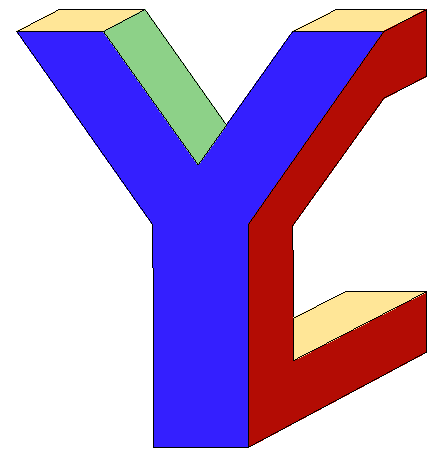
\includegraphics[height=1.5cm]{pictures/YC_logo.pdf}
    \end{center}
    &
    \begin{center}
      
\includegraphics[height=1.5cm]{pictures/SPbGU_Logo.png}
    \end{center}
  \end{tabular}
  \titlepage
\end{frame}
}

\begin{frame}[fragile] \frametitle{Зиннатулин Тимур Раифович}
      \begin{minipage}[m]{0.45\linewidth}
  \raisebox{-0.5\totalheight}{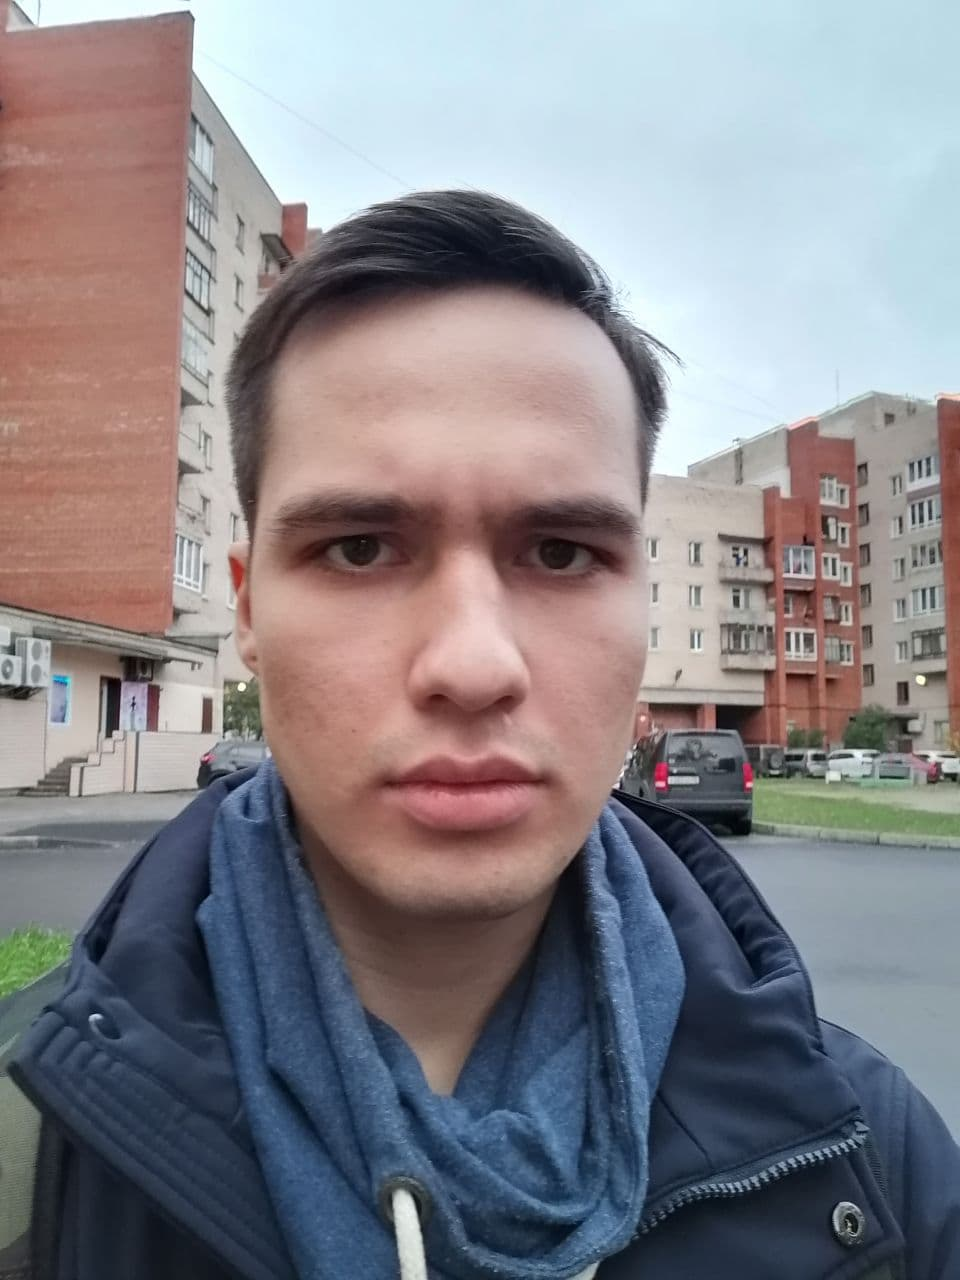
\includegraphics[width=\textwidth]{pictures/Zinnatulin_ProfilePhoto.jpg}}
  \end{minipage}\hfill
  \begin{minipage}[m]{0.54\linewidth}
  \vspace{-2cm}
  Кандидат на бакалаврский грант

  \begin{itemize}
        \item Работает с нами с сентября 2019 года (2 курс, семестровый проект)
        \item Закончит третий курс Мат-Мех факультета в июне 2021 года
        \item Тема курсовой работы: ``Реализация поиска путей с регулярными и контекстно-свободными ограничениями в графовой базе данных RedisGraph''
        \item Получатель стипендии        
  \end{itemize}
  \end{minipage}

\end{frame}


            


\begin{frame}[fragile] \frametitle{Исследовательская работа}
  
    \begin{itemize}
        \item Сфера интересов: алгоритмы выполнения запросов в графовых базах данных
        \item Соавтор одной опубликованной работы: ``Multiple-Source Context-Free Path Querying in Terms of Linear Algebra''. Arseniy Terekhov, Vlada Pogozhelskaya, Rustam Azimov, Vadim Abzalov, \textbf{Timur Zinnatulin}, Semyon Grigorev; 2021; International Conference on Extending Database Technology (EDBT)        
        \item Реализовал поддержку запросов с КС ограничениями в синтаксисе Cypher для RedisGraph
    \end{itemize}
  \pause
  \vfill
  Планы: экспериментальное исследование алгоритмов решения задачи достижимости с контекстно-свободными ограничениями, основанных на линейной алгебре
  \begin{itemize}
        \item Сравнение RedisGraph с другими графовыми БД на регулярных запросах
        \item Сравнение RedisGraph с другими графовыми БД и самостоятельными инструментами на КС запросах в рамках задачи статического анализа кода
        \item Публикация результатов экспериментального исследования
  \end{itemize}

\end{frame}


\begin{frame}[fragile] \frametitle{Панфилёнок Дмитрий Викторович}
      \begin{minipage}[m]{0.45\linewidth}
  \raisebox{-0.5\totalheight}{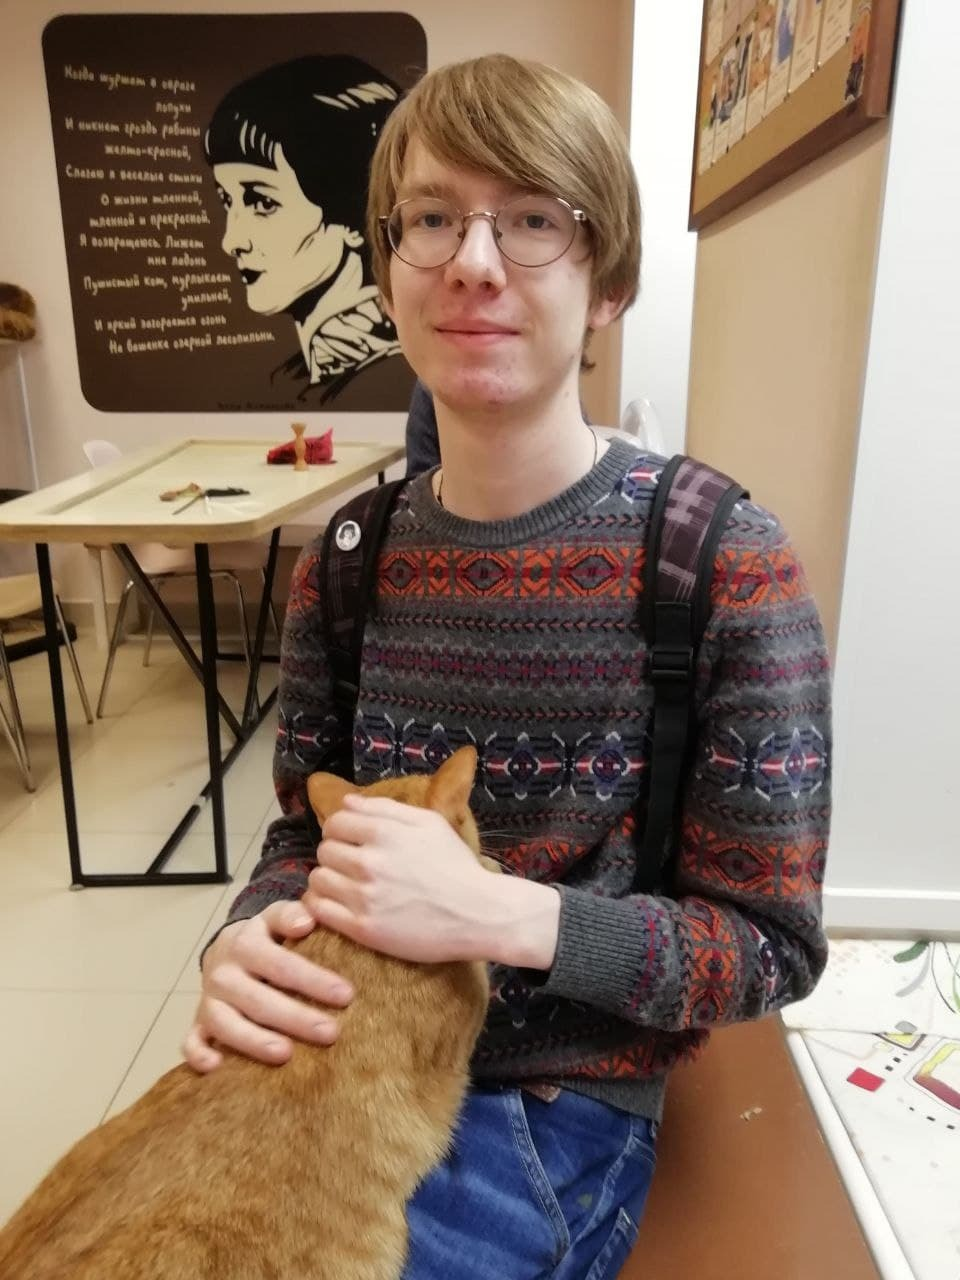
\includegraphics[width=\textwidth]{pictures/Panfilyonok_ProfilePhoto.jpg}}
  \end{minipage}\hfill
  \begin{minipage}[m]{0.54\linewidth}
  \vspace{-2cm}
  Кандидат на бакалаврский грант

  \begin{itemize}
        \item Работает с нами с сентября 2020 года (курсовая 3 курса)
        \item Закончит третий курс Мат-Мех факультета в июне 2021 года
        \item Тема курсовой работы: ``Реализация GraphBLAS API для матриц в CSR формате на платформе OpenCL с использованием F\#''
        \item Получатель стипендии
  \end{itemize}
  \end{minipage}

\end{frame}


\begin{frame}[fragile] \frametitle{Исследовательская работа}
  
    \begin{itemize}
        \item Сфера интересов: системное программирование (решение инженерных задач), функциональное программирование, биоинформатика
        \item Начата работа над публикацией об опыте реализации GraphBLAS API на функциональном языке программирования        
    \end{itemize}
  \pause
  \vfill
  Планы: разработка и экспериментальное исследование высокоуровневых средств разработки для GPGPU на примере реализации подмножетсва GraphBLAS API
  \begin{itemize}
        \item Улучшение средства разработки для GPGPU на языке программирования F\# (Brahma.FSharp)
        \item Реализация подмножества GraphBLAS API с использованием Brahma.FSharp
        \item Проведение экспериментального исследования полученной реализации, сравнение с аналогами
        \item Публикация результатов (GrAPL-2022)
  \end{itemize}

\end{frame}


\begin{frame}[fragile] \frametitle{Погожельская Влада Владимировна}
      \begin{minipage}[m]{0.45\linewidth}
  \raisebox{-0.5\totalheight}{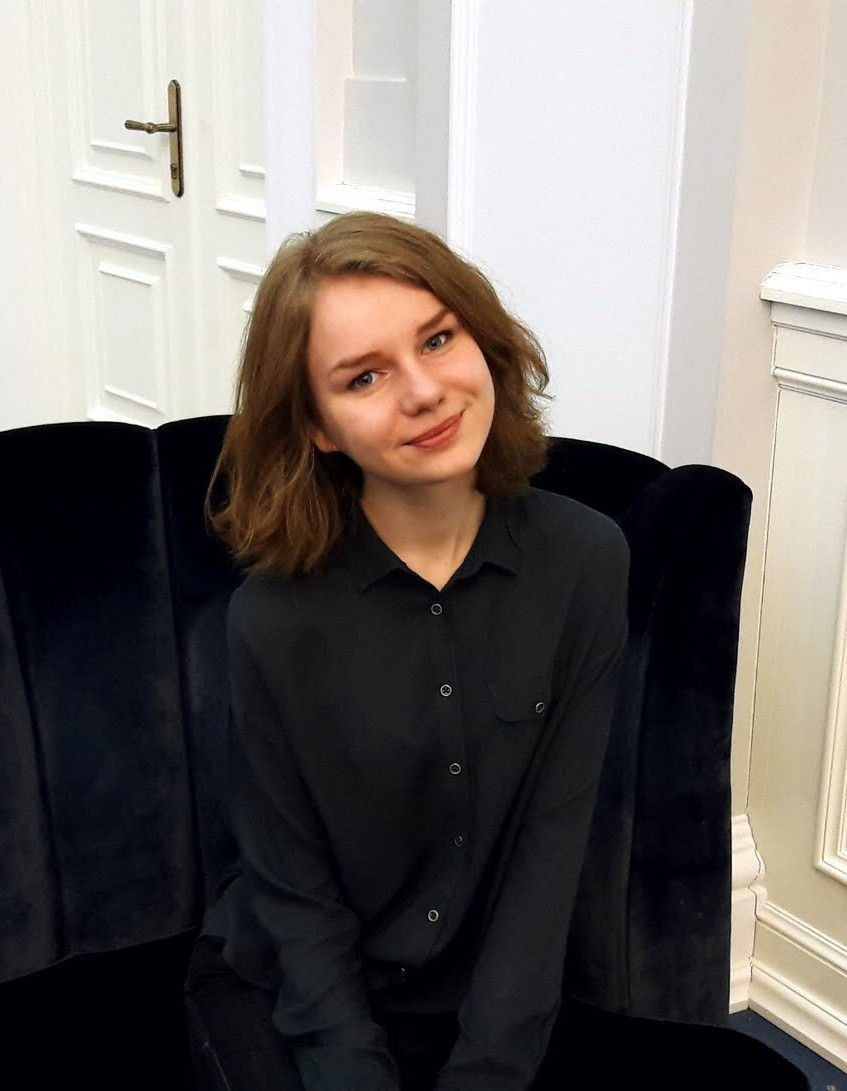
\includegraphics[width=\textwidth]{pictures/Pogozelskaia_ProfilePhoto.jpg}}
  \end{minipage}\hfill
  \begin{minipage}[m]{0.54\linewidth}
  \vspace{-2cm}
  Кандидат на бакалаврский грант

  \begin{itemize}
        \item Работает с нами с сентября 2019 года (2 курс, семестровый проект)
        \item Закончит третий курс Мат-Мех факультета в июне 2021 года
        \item Тема курсовой работы: ``Улучшение производительности алгоритма поискапутей с контекстно-свободными ограничениями дляграфовой базы данных Neo4j''
        \item Получатель стипендии        
  \end{itemize}
  \end{minipage}

\end{frame}


\begin{frame}[fragile] \frametitle{Исследовательская работа}
  
    \begin{itemize}
        \item Сфера интересов: алгоритмы выполнения запросов в графовых базах данных
        \item Соавтор одной опубликованной работы: ``Multiple-Source Context-Free Path Querying in Terms of Linear Algebra''. Arseniy Terekhov,  \textbf{Vlada Pogozhelskaya}, Rustam Azimov, Vadim Abzalov,Timur Zinnatulin, Semyon Grigorev; 2021; International Conference on Extending Database Technology (EDBT)        
        \item Работает над реализацией алгоритма выполнения запросов с КС ограничениями в Neo4j на основе GLL
    \end{itemize}
  \pause
  \vfill
  Планы: экспериментальное исследование решения для поиска путей с КС и регулярными ограничениями в Neo4j на основе GLL
  \begin{itemize}
        \item Сравнение Neo4j с другими графовыми БД на регулярных запросах
        \item Сравнение Neo4j с другими графовыми БД и самостоятельными инструментами на КС запросах в рамках задачи статического анализа кода
        \item Публикация алгоритма и результатов экспериментального исследования
  \end{itemize}

\end{frame}


\begin{frame}[fragile] \frametitle{Абзалов Вадим Игоревич}
      \begin{minipage}[m]{0.45\linewidth}
  \raisebox{-0.5\totalheight}{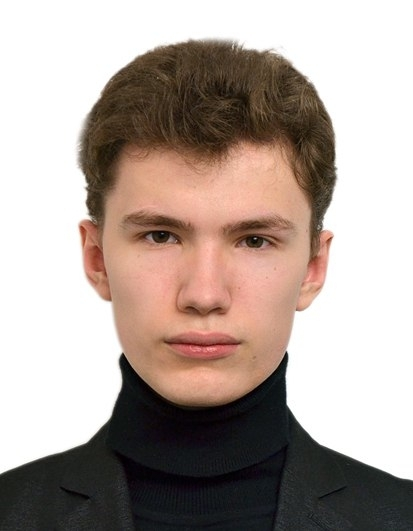
\includegraphics[width=\textwidth]{pictures/Abzalov_ProfilePhoto.jpg}}
  \end{minipage}\hfill
  \begin{minipage}[m]{0.54\linewidth}
  \vspace{-2cm}
  Кандидат на бакалаврский грант

  \begin{itemize}
        \item Работает с нами с сентября 2019 года (2 курс, семестровый проект)
        \item Закончит третий курс Мат-Мех факультета в июне 2021 года
        \item Тема курсовой работы: ``Модернизация набора данных CFPQ\_Data''
        \item Получатель стипендии        
  \end{itemize}
  \end{minipage}

\end{frame}


\begin{frame}[fragile] \frametitle{Исследовательская работа}
  
    \begin{itemize}
        \item Сфера интересов: графовые базы данных, машинное обучение, биоинформатика
        \item Соавтор одной опубликованной работы: ``Multiple-Source Context-Free Path Querying in Terms of Linear Algebra''. Arseniy Terekhov, Vlada Pogozhelskaya, Rustam Azimov, \textbf{Vadim Abzalov}, Timur Zinnatulin, Semyon Grigorev; 2021; International Conference on Extending Database Technology (EDBT)        
        \item Основной разработчик проекта \href{https://github.com/JetBrains-Research/CFPQ_Data}{CFPQ\_Data}
    \end{itemize}
  \pause
  \vfill
  Планы: улучшение качества предсказания вторичной структуры РНК на основе синтаксического анлиза и свёрточных нейронных сетей
  \begin{itemize}
        \item Публикация по собранному в рамках курсовой набору данных
        \item Эксперименты с решением Полины Луниной, его улучшение (доработка граммтики, улучшение алгоритма синтаксического анализа, улучшение модели)
        \item Публикация результатов совместно с Полиной Луниной
  \end{itemize}

\end{frame}


\end{document}
